\thispagestyle{lichsutoanhocnone}
\pagestyle{lichsutoanhoc}
\graphicspath{{../lichsutoanhoc/pic2/}}
\everymath{\color{lichsutoanhoc}}
\blfootnote{$^1$\color{lichsutoanhoc}THPT chuyên Hà Nội -- Amsterdam.}
\begingroup
\AddToShipoutPicture*{\put(0,616){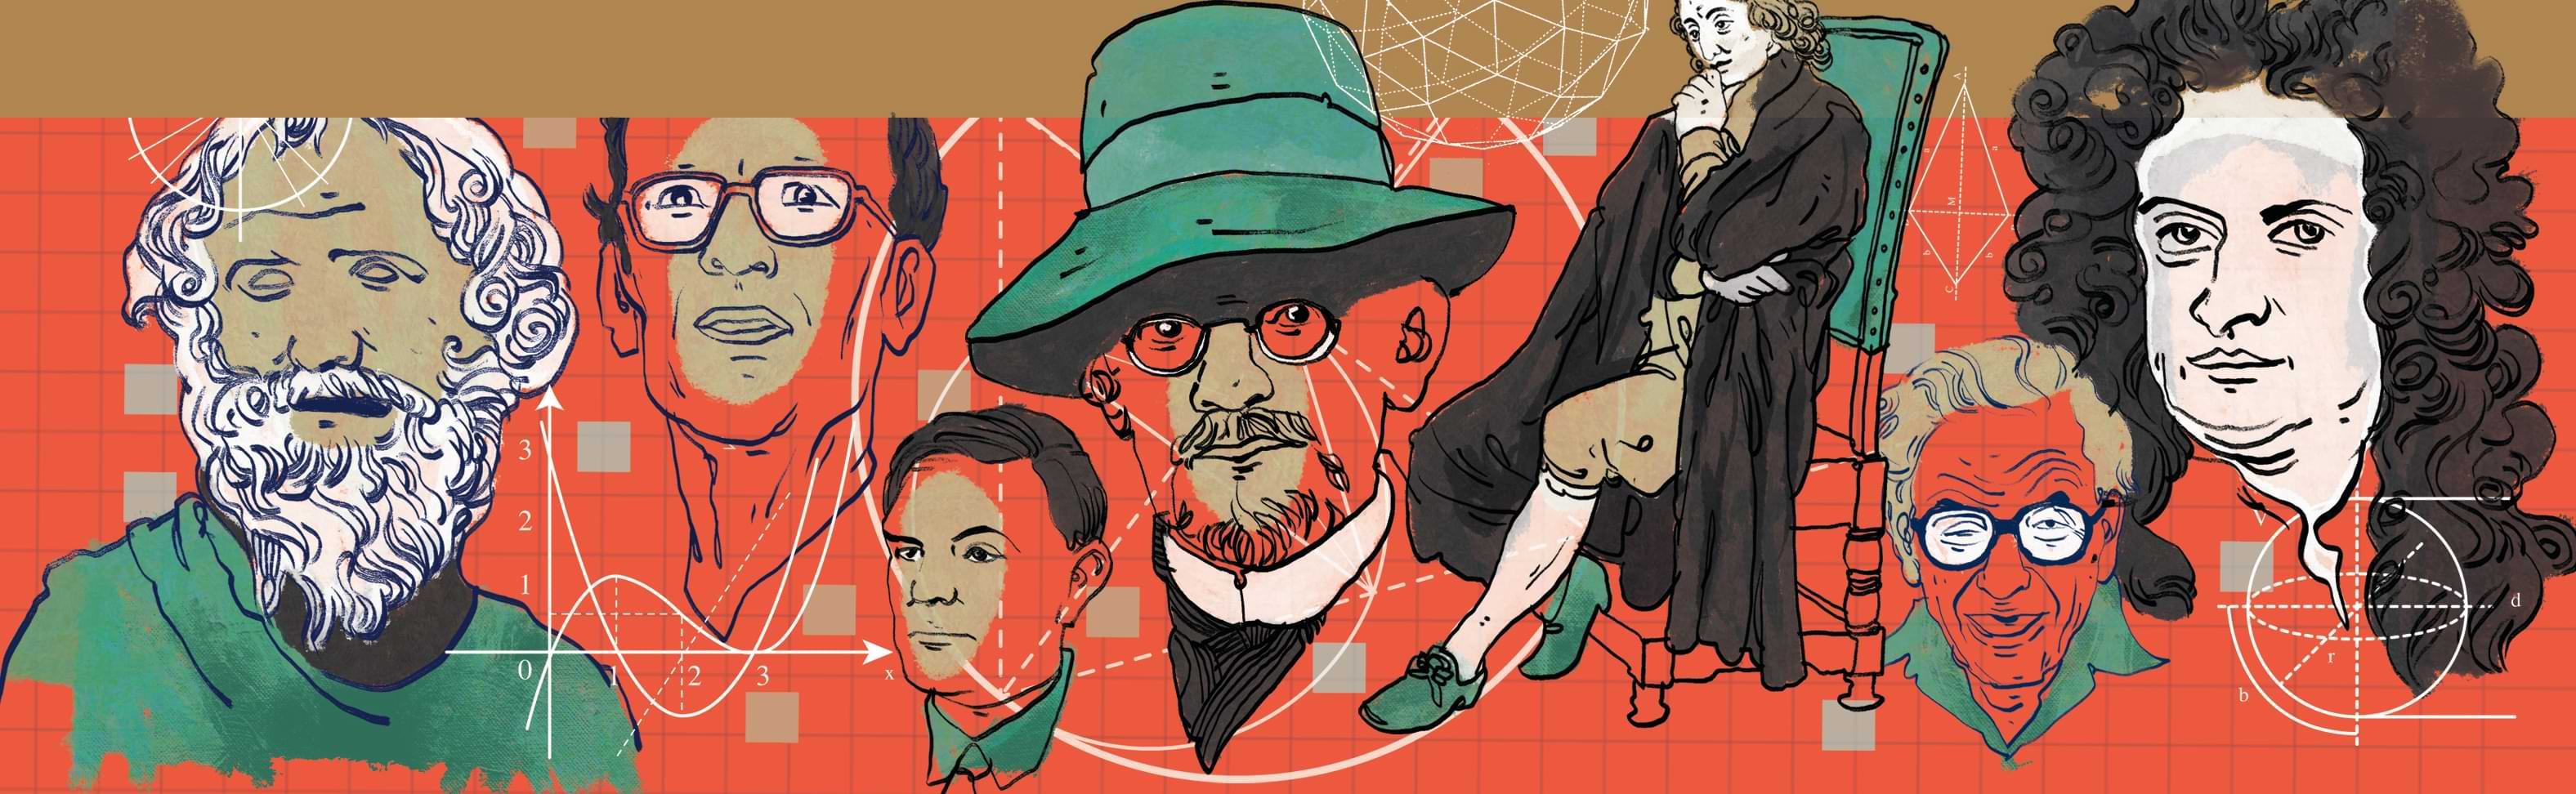
\includegraphics[width=19.3cm]{../bannerlichsu}}}
\AddToShipoutPicture*{\put(120,522){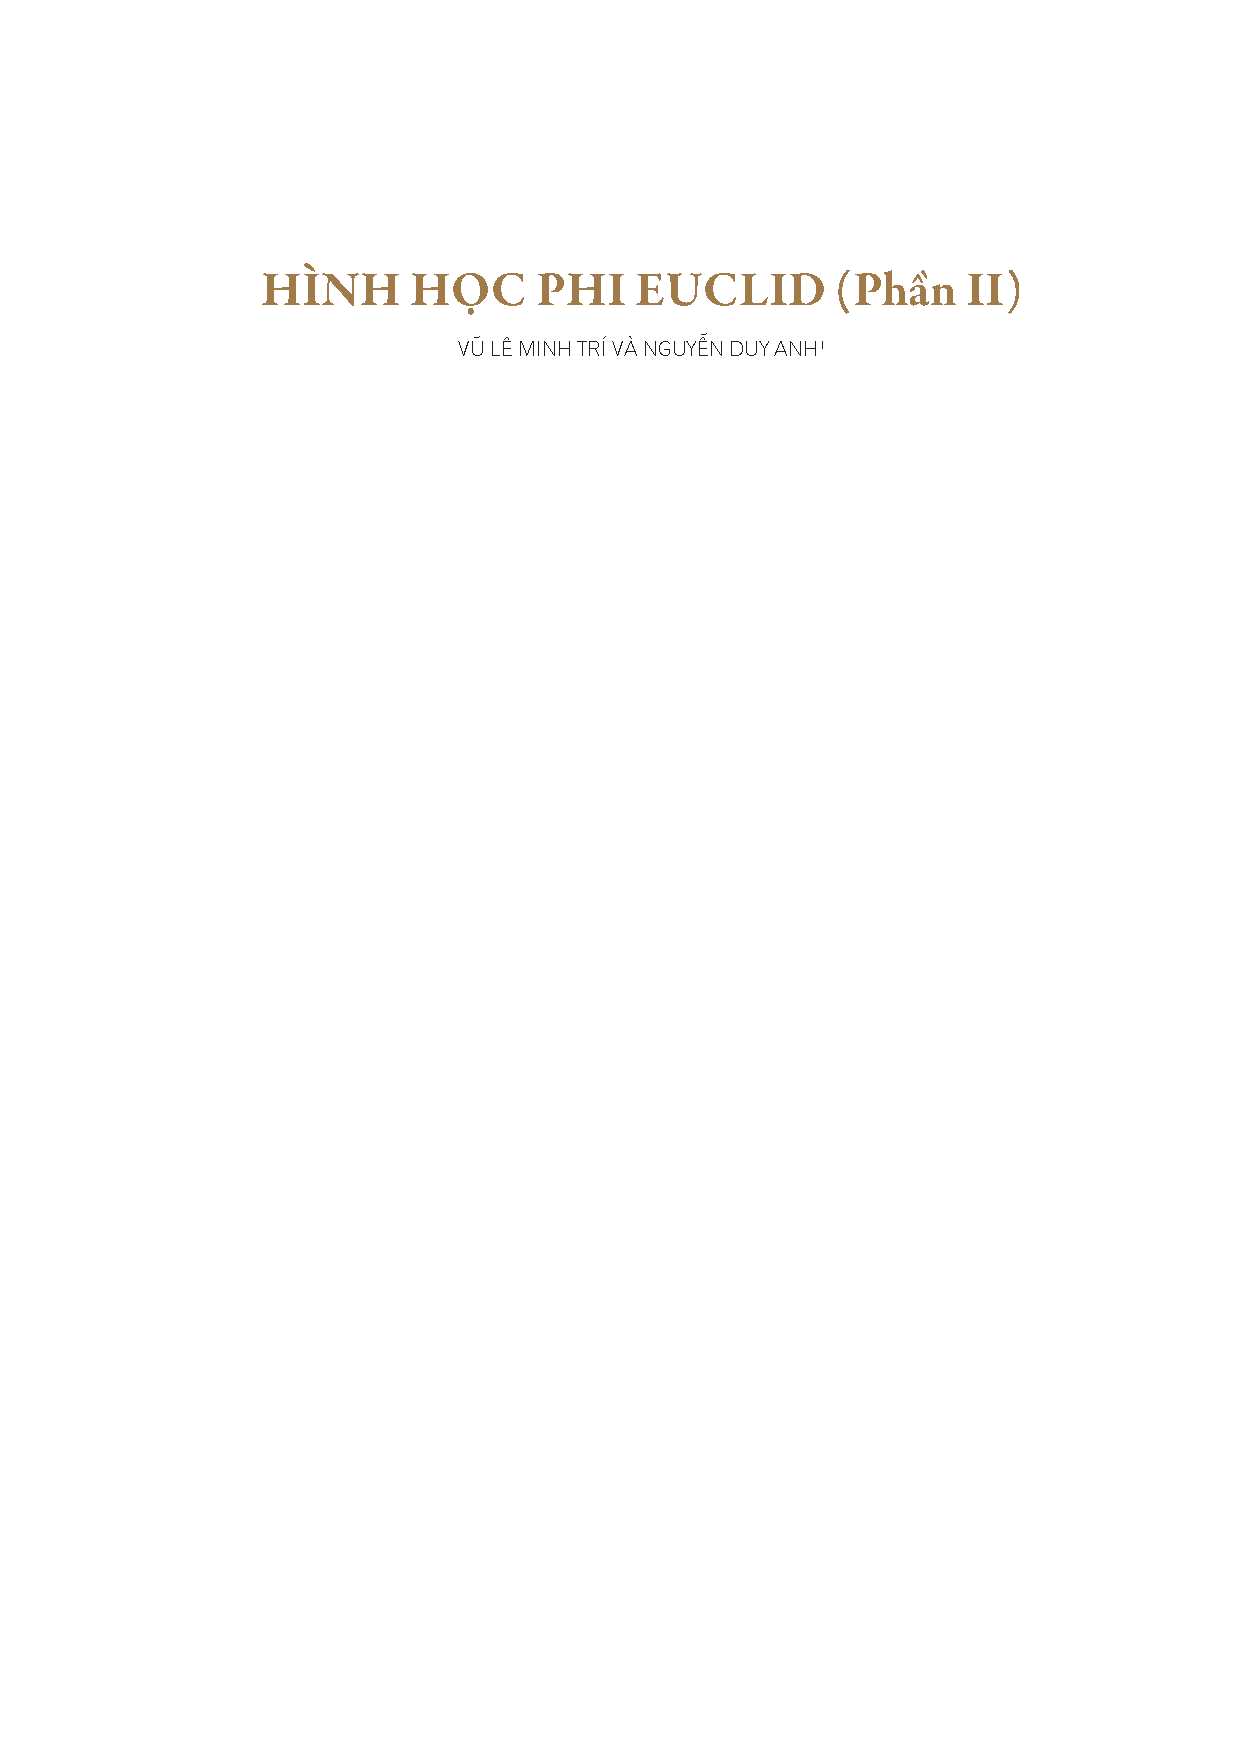
\includegraphics[scale=1]{../tieude3.pdf}}}
\centering
\endgroup

\vspace*{185pt}

\begin{multicols}{2}
	Một ý tưởng tưởng chừng như mâu thuẫn với những cảm quan thường thức, thế nhưng lại trở thành một vũ trụ hình học mới lạ và chặt chẽ, và có thể nắm giữ bản chất của không gian chúng ta đang sống. Thế nhưng quá trình khám phá và phát triển ý tưởng ấy phải trải qua hàng thập kỷ với nhiều trắc trở và gian nan.
	\vskip 0.1cm
	\textbf{\color{lichsutoanhoc}Những nhà tiên phong}
	\vskip 0.1cm
	Tiếc cho Saccheri khi tác phẩm giá trị của ông không nhận được sự chú ý của nhiều người hơn, vì thế nên câu hỏi về Tiên đề $5$ của Euclid vẫn còn dai dẳng tới tận cả thế kỷ sau. Và số phận lần nữa lại trêu ngươi các nhà Toán học, khi mà không phải một, mà tận ba người đã gần như cùng lúc đến với đáp án cho câu hỏi lớn của chúng ta. Dù vậy, cách tiếp cận vấn đề của họ khác nhau một trời một vực.
	\vskip 0.1cm
	Carl Friedrich Gauss là một trong những nhà Toán học vĩ đại nhất mọi thời đại. Trong suốt chiều dài sự nghiệp, ông đã để lại những công trình vượt xa tri thức thời ấy trong rất nhiều lĩnh vực như lý thuyết số, lý thuyết xác suất, hình học và lý thuyết hàm số. Khác với những Leonhard Euler hay Augustin Louis Cauchy xuất bản vô cùng tích cực, Gauss tuân thủ triết lý ``Ít nhưng chín" (pauca sed matura): chỉ khi nào ông suy ngẫm đến mức đủ thấu đáo theo ý ông, và chỉ khi ông đã trình bày súc tích vấn đề ấy, ông mới cho đăng một nghiên cứu nào đó. Những ý tưởng ``chưa đủ chín" được ông tập hợp lại trong ngăn bàn làm việc, nơi mà dần dà tích trữ lượng tri thức đi trước thời đại $50$ năm. Khi Gauss bàn luận về Toán, thường sẽ có một tập giấy trong đó có ích cho cuộc trao đổi, được lấy ra sau câu cửa miệng ``tôi cũng đã suy nghĩ về vấn đề đó rồi", đôi lúc kèm theo ``tôi cũng đã đạt đến những kết quả tương tự".
	\vskip 0.1cm
	Không lĩnh vực Toán nào là Gauss không chạm tới, và câu hỏi về tiên đề thứ $5$ không phải ngoại lệ. Nhà Toán học vĩ đại đã trăn trở về vấn đề này từ năm lên $15$, và sau nhiều thất bại, ông dần nghi ngờ sự tồn tại của một chứng minh. Cũng như những người đi trước, ông đã thử giả sử phản chứng Tiên đề $5$, cũng khám phá ra nhiều kết quả mà chưa thấy mâu thuẫn xuất hiện. Ông chưa vội xuất bản gì về những phát hiện ấy, mà tự mình tìm tòi trong đó cho đến khi bản thân ông đã hài lòng. Ngoài phương châm xuất bản của bản thân, còn một thế lực khác khiến ông dè dặt. Chả là có một người đồng hương đương thời có ảnh hưởng chẳng kém cạnh Gauss chút nào đã lên tiếng -- triết gia Immanuel Kant. Kant đồng ý rằng kiến thức bắt đầu từ những trải nghiệm từ bên ngoài, nhưng cho rằng trí óc có thể hành động dựa trên những ấn tượng chỉ có thể là bởi nó đã có những ``trực giác" về không gian và thời gian độc lập với kinh nghiệm, và cũng đúc khuôn những kinh nghiệm ấy. ``Khái niệm của không gian Euclid không có nguồn gốc thực nghiệm nào cả, mà là sự cần thiết không thể tránh khỏi của suy nghĩ. Không hệ thống hình học nào khác tồn tại, vì không hệ thống hình học nào khác có thể được hình dung.", Kant viết.
	\vskip 0.1cm
	Riêng khẳng định vừa rồi là sai, bởi các nhà Toán học đã hiểu được phần nào lời giải của vấn đề về Tiên đề $5$, và sắp tới thì hi vọng là quý độc giả cũng vậy. Về phần Gauss, do sự đông đảo của các tín đồ theo Kant và những ``người hâm mộ" Euclid, ông tránh né gây hấn với họ, có nghĩa là ông không xuất bản các phát hiện của mình. Tất nhiên Gauss không chỉ có một mình, mà một bằng hữu của ông sẽ có đóng góp lớn vào các sự kiện sắp tới.
	\vskip 0.1cm
	Farkas Bolyai ($1775-1856$) là nhà toán học người Hungary, ban đầu học ở Jena, về sau trở thành đồng môn và một người bạn gần gũi của Gauss khi hai người học ở Gottingen. Mối quan hệ này được họ duy trì suốt phần đời còn lại. 
	\vskip 0.1cm
	Sau nhiều nỗ lực và tâm sức, Bolyai đã nhận ra một điều đáng chú ý về tiên đề song song: ông không thể chứng minh được nó mà không ngộ nhận. Có một lần người bạn Gauss còn giúp ông nhận ra sai sót của mình trong một chứng minh bất thành. Là một nhà toán học khá xuất sắc, với một tác phẩm nổi tiếng về Toán sơ cấp, Tentamen Juventutem Studiosam in Elementa Matheseos Purae (tạm dịch ``Nỗ Lực Giới Thiệu Những Yếu Tố của Toán Thuần Túy tới Thanh niên Ham học"), thế nhưng danh tiếng của Farkas Bolyai hầu như đến từ việc ông là \ldots cha của con ông, Janos Bolyai. 
	\begin{figure}[H]
		\vspace*{5pt}
		\centering
		\captionsetup{labelformat= empty, justification=centering}
		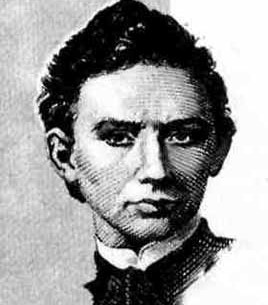
\includegraphics[width= 1\linewidth]{JanosBolyai}
		\caption{\small\textit{\color{lichsutoanhoc}Janos Bolyai, lấy từ tem của Bưu điện Hungary, nhân kỷ niệm $100$ năm ngày mất. Hai bức hình gốc của cậu đều đã thất lạc.}}
		\vspace*{-10pt}
	\end{figure}
	Janos ($1802-1860$) từ sớm đã tỏ ra là một nhà toán học uyên bác hơn cả cha mình. Đơn cử như khi Farkas đổ bệnh, ông đã cho cậu con trai mới $13$ tuổi đứng lớp thay. Không muốn uổng phí tiềm năng của cậu quý tử, Bolyai cha đã gửi thư cho Gauss nhờ ông thu nhận Janos, nhưng oái oăm thế nào mà chẳng được hồi đáp sau tận $16$ năm. Vì thế chàng trai trẻ đã rẽ ngang sang học ở Viện Kỹ Thuật Hoàng Gia tại Vienna năm $1817$, và đi theo quân đội sau khi tốt nghiệp. Trong $10$ năm sau đó, Janos không chỉ là một nhà toán học sâu sắc, mà còn là một nghệ sĩ violin say mê, và một chuyên gia đấu kiếm. Cậu từng chấp nhận lời thách thức đấu kiếm với $13$ sĩ quan kỵ binh, với điều kiện là cậu được chơi violin sau mỗi $2$ trận đấu. Kết quả là $13-0$ cho Janos.
	\vskip 0.1cm
	May cho chúng ta, và ban đầu là không may lắm cho người cha Farkas, chàng thanh niên Janos tài năng cũng bị bài toán chứng minh Tiên đề $5$ hớp hồn, rồi lao vào nghiên cứu. Cha cậu ngậm ngùi nhớ lại kết cục ông từng trải, nhắn gửi cậu những lời sau đây:
	\vskip 0.1cm
	``Đừng dành một giờ đồng hồ nào cho vấn đề đó (tiên đề song song). Nó không đưa đến một kết quả nào cả; thay vào đó nó sẽ đầu độc cả cuộc đời con \ldots Ta tin rằng bản thân ta đã tìm ra mọi ý tưởng có thể nghĩ tới liên quan đến vấn đề này."
	\vskip 0.1cm
	Trái với mong muốn của cha, Janos được tiếp thêm động lực để tiếp tục, nhưng rồi chuỗi bất bại $2000$ năm của bài toán ấy cũng dần khiến cậu nghĩ rằng tiên đề số $5$ thực sự không phải định lý. Và cậu cũng chọn đi con đường giả sử phản chứng, tiếp tục đào sâu vào thứ Hình học xa lạ giờ đây đang dần được cậu định hình rõ nét. Khác với Saccheri, cậu chẳng vướng bận với nghĩa vụ chứng minh Euclid là đúng; trong mắt chàng trai trẻ, thế giới mới này rực rỡ chẳng kém gì thứ hình học được tôn sùng bấy lâu. Thành quả của cậu khiến chính người cha thay đổi quan niệm. ``Từ hư không, con đã tạo ra một vũ trụ lạ lẫm và mới mẻ", Janos khẳng định trong một bức thư trao đổi với cha. 
	\begin{figure}[H]
		\vspace*{-5pt}
		\centering
		\captionsetup{labelformat= empty, justification=centering}
		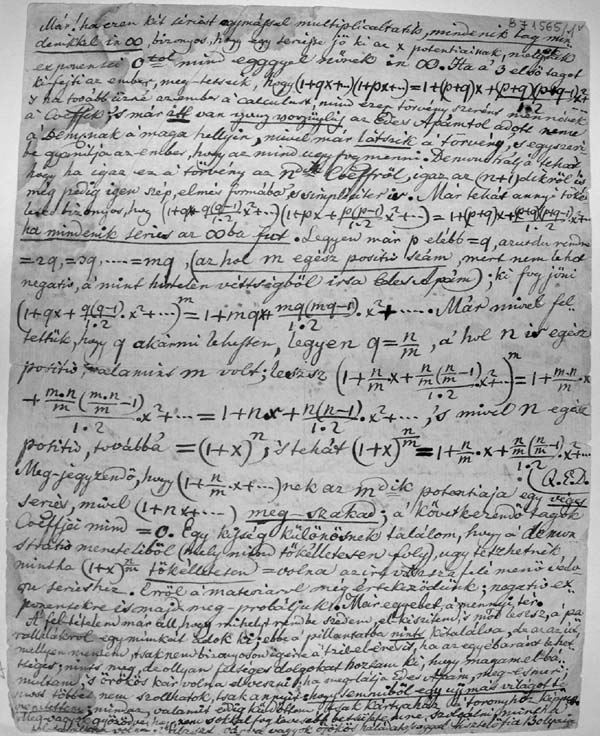
\includegraphics[width= 1\linewidth]{Bolyai_letter_2}
		\caption{\small\textit{\color{lichsutoanhoc}Dòng được gạch chân ở cuối trang: ``Từ hư không, con đã tạo ra một vũ trụ lạ lẫm và mới mẻ".}}
		\vspace*{-10pt}
	\end{figure}
	Farkas hí hửng thêm những kết quả ấy vào trong cuốn ``Tentamen" lần tái bản năm $1832$, dưới tiêu đề Appendix Scientiam Spatii Absolute Veram Exhibens (Phụ lục Giải thích Khoa học Tuyệt đối của Không gian), đồng thời nối lại liên lạc với cây đa cây đề Gauss của Toán học đương thời. Gauss hết lời tán dương, song lại có đoạn ông viết:
	\vskip 0.1cm
	``Nếu tôi bắt đầu với việc nói rằng tôi không dám khen ngợi công trình này, hẳn trong một khắc anh sẽ ngạc nhiên, nhưng tôi không thể làm khác. Khen ngợi nó đồng nghĩa với việc khen ngợi chính tôi. Vì toàn bộ nội dung của công trình, từ cả hướng tiếp cận của con trai anh, tới cả những kết quả mà nó thu được, trùng khớp gần như hoàn toàn những suy nghĩ đã chiếm giữ đầu óc tôi suốt ba mươi hay ba mươi lăm năm qua \ldots Kế hoạch của tôi là viết tất cả ra giấy, để ít nhất thì những ý tưởng này không theo tôi xuống mồ. Nên tôi rất ngạc nhiên khi có người đã làm việc này thay tôi, và đặc biệt vui mừng khi người đó lại chính là con trai của người bạn cũ đã vượt xa tôi một cách ấn tượng đến vậy."
	\vskip 0.1cm
	Đoạn thư này với Janos như là Gauss khẳng định ông lấy cắp ý tưởng của cậu. Thật ra, những kết quả cậu (và nhân vật thứ ba mà chúng ta sắp nói đến) đạt được chi tiết và phong phú hơn Gauss rất nhiều, điều này chính Gauss còn công nhận. Vốn tính khí nóng nảy, cậu trai thất vọng kinh khủng, và khoảnh khắc ấy là lúc cậu đoạn tuyệt với xuất bản (hên cho hậu thế là khoảng $20000$ trang bản thảo của Janos vẫn còn). Dù về sau đã dẹp bỏ được mối nghi ngờ về nhà Toán học lão thành, Janos vẫn chẳng thể vực dậy tinh thần bản thân do công trình của cậu chẳng hề được người đời hưởng ứng. Đạp đổ một tượng đài trong lòng nhân loại suốt hai thiên nhiên kỷ chẳng phải dễ dàng, và điều ấy càng khắc sâu nỗi thất vọng vốn có. Sự công nhận xứng đáng cho Janos đáng tiếc lại không đến khi cậu còn sống.
	\vskip 0.1cm
	Quay ngược thời gian về năm $1829$, $3$ năm trước bài báo của Janos, một bài báo về chủ đề tương tự đã xuất hiện tại nước Nga xa xôi. Tác giả là nhân vật chính thứ ba, Nikolai Lobachevsky. 
	\begin{figure}[H]
		\vspace*{-5pt}
		\centering
		\captionsetup{labelformat= empty, justification=centering}
		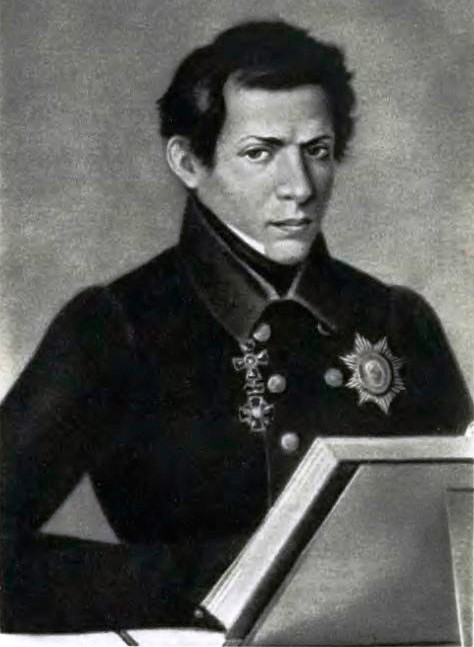
\includegraphics[width= 1\linewidth]{Lobachevsky_03_crop}
		\caption{\small\textit{\color{lichsutoanhoc}Nikolai Ivanovich Lobachevski.}}
		\vspace*{-10pt}
	\end{figure}
	Nói qua về bối cảnh giáo dục Nga thời ấy. Giáo dục nói chung và Toán học nói riêng ở Nga giai đoạn cuối thế kỷ $18$ -- đầu thế kỷ $19$ chưa được phát triển như các quốc gia phương Tây khác. Tình hình không khả quan hơn sau khi cuộc chinh phạt của Napoleon đại đế sa lầy giữa mùa đông nước Nga, bởi sự kiện này đã làm dậy lên hai hiện tượng trong lòng người dân Nga thời bấy giờ: họ dần có ác cảm với những ảnh hưởng ngoại bang, và niềm tin vào một Đấng tối cao thần bí cứu rỗi mẫu quốc Nga vĩ đại được nhen nhóm lại mạnh mẽ, không tốt cho phát triển khoa học. Đứng trước hai cơn gió ngược chiều, công cuộc cường hóa nền giáo dục nước nhà, lấy ấy làm tiềm lực quốc gia của Sa Hoàng Aleksandr chẳng hề thuận lợi. Lobachevsky đến tuổi vào Đại học Kazan trong bối cảnh đó, và sẽ dành $40$ năm cuộc đời ông gắn bó với nơi đây.
	\vskip 0.01cm
	Chẳng rõ tự bao giờ, Lobachevsky đã nghiền ngẫm và thử đưa ra những chứng minh, cũng đã nghi ngờ và thử giả sử mệnh đề phủ định của tiên đề song song, và cũng đã theo mạch phát triển mà chẳng thấy mâu thuẫn nào. Đến lúc ấy, hẳn Lobachevsky đã bị thuyết phục bởi lượng kết quả mới quá nhiều để có thể dẫn đến một mâu thuẫn, ông dành tận ba năm phát triển hệ thống ông mới tạo dựng. Ông cho xuất bản những kết quả của mình trên tờ ``Messenger" của Kazan, và chỉ nhận lại cái quay lưng lạnh nhạt của giới học thuật. Ngoài việc nền giáo dục Nga xa cách với các trung tâm sôi nổi của cộng đồng nghiên cứu, điều này một phần còn do Lobachevsky đặt tên loại hình học này là ``hình học tưởng tượng" (imaginary geometry). Bài báo ``Về Nền tảng của Hình học" của ông còn bị từ chối bởi một reviewer thờ ơ thuộc Viện Hàn lâm Khoa học St. Petersburg, với lý do hai tích phân xác định trong bài báo thì một cái là sai, cái còn lại thì dễ chứng minh. Sở dĩ một bài báo về hình học có yếu tố giải tích là bởi Lobachevsky đã phát triển lượng giác của loại hình học này.
	\vskip 0.1cm
	Lobachevsky không vì phản ứng của dư luận mà nhụt chí. Ông ra sức viết hàng loạt bài báo để thuyết phục giới học thuật về tầm cỡ của thành tựu của ông. Ông vẫn hết mình với ngôi trường ông giảng dạy, hết mình với lao động. Khi trao đổi những kết quả với Gauss, ông nhận lại những lời khen có cánh, thậm chí là lời đề nghị ông giữ một chân tại khoa Toán Đại học Gottingen cạnh Gauss. Lobachevsky từ chối. Trong suốt những năm tháng gắn bó với Đại học Kazan, Lobachevsky đã kiêm vai trò của giảng viên, nhà nghiên cứu, thành viên hội đồng quản trị, lao công, thậm chí từng thiết kế kiến trúc và giúp trường chống dịch tả.
	\vskip 0.1cm
	Đáp lại những công lao đó, trung ương đã hào phóng tặng một Lobachevsky đã ngoài ngũ tuần một lượt về hưu non. Có người cho rằng, những thế lực khiến Gauss e ngại đã nhúng tay vào: những tín đồ của Euclid và Kant hẳn đã rỉ tai gia đình hoàng tộc về thứ hình học mới đã xúc phạm đến tượng đài tri thức của  Hy Lạp và Euclid. Kể cả quyết định đột ngột trên, hay nỗi đau mất con, hay sự mù lòa sau này, tất cả vẫn chẳng thể quật ngã Lobachevsky, ông vẫn nghiên cứu về loại hình học phủ định tiên đề song song chừng nào ông còn nghĩ được, vẫn nhiều lần xuất bản thêm đến cuối đời. Vào kỷ niệm $50$ năm thành lập Đại học Kazan, ông lại cho đăng tải một bài báo về công trình để đời ông, lúc này được ông gọi là Pangeometry. Đổi tên vẫn không giúp ông nhận được sự công nhận xứng đáng.
	\vskip 0.1cm
	Cùng một bài toán ta có ba cách tiếp cận: người thì giữ làm bí mật do lo sợ thời thế, người lại cay đắng thất vọng sau một bức thư, người lại chẳng hề ngán bất cứ điều gì, vững tin vào thành quả bản thân. Dù gì đi nữa thì những công trình hết sức công phu của họ đã khiến dư luận dần có lý do để tin:
	\vskip 0.1cm
	\textit{Tiên đề song song không thể được chứng minh từ các tiên đề còn lại} 
	\vskip 0.1cm
	$\pmb{2.}$ \textbf{\color{lichsutoanhoc}Sự phi mâu thuẫn}
	\vskip 0.1cm
	Tuy nhiên có một điều cả $3$ người tiên phong trên thiếu. Loại hình học họ nghĩ ra vẫn thuần túy ``nằm trên giấy", sự phi mâu thuẫn của nó vẫn chỉ là giả định. Hình dung hậu thế dốc sức phát triển hàng trăm định lý, để rồi ai đó phát hiện ra một mâu thuẫn quá đỗi đơn giản nào đó. Mà từ các mệnh đề mâu thuẫn, người ta có thể chứng minh được mọi mệnh đề, nên một hệ tiên đề chứa mâu thuẫn chắc chắn là không đem lại giá trị gì. Nhiệm vụ cấp thiết tiếp theo chính là chứng minh sự phi mâu thuẫn đó.
	\vskip 0.1cm
	Mọi nghi ngờ cuối cùng cũng được giải quyết bởi Eugenio Beltrami ($1835-1900$) vào năm $1868$ (người đàn ông này cũng giới thiệu lại công trình bị bỏ quên của Saccheri): hình học Euclid và loại hình học mới mẻ này ``đúng như nhau". 
	\begin{figure}[H]
		\vspace*{5pt}
		\centering
		\captionsetup{labelformat= empty, justification=centering}
		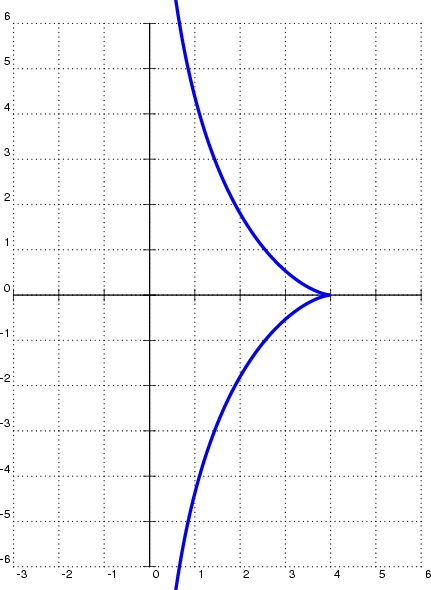
\includegraphics[width= 1\linewidth]{Tractrix.png}
		\caption{\small\textit{\color{lichsutoanhoc}Đường cong Tractrix.}}
		\vspace*{-10pt}
	\end{figure}
	Cách làm rất đơn giản: dựng ra một không gian tuân theo quy luật của hình học mới trong chính không gian của hình Euclid. Và mô hình mà Beltrami lựa chọn là bề mặt của một ``ngụy cầu" (pseudosphere), thứ mà ta thu được khi ta quay một đường cong tractrix xung quanh trục hoành. Nếu định nghĩa đường thẳng trên bề mặt này là đường đi ngắn nhất giữa $2$ điểm, thì một phần các tính chất hình học trên bề mặt này thỏa mãn hình học của Bolyai và Lobachevsky. 
	\vskip 0.1cm
	Quan trọng hơn, mọi định lý của loại hình học trên bề mặt này có thể được quy về một định lý tương ứng trong hình học Euclid, tức là nếu hình học mới này có mâu thuẫn, thì hình học của Euclid cũng vậy. Nói cách khác, hình học Euclid, thứ ở vị trí thống trị suốt từ thời Hy Lạp cổ đại đến lúc ấy, chỉ ``đúng ngang với" hình học mới của Gauss, Bolyai và Lobachevsky mà thôi. Phần phân tích hai mô hình Beltrami--Klein và Poincaré sẽ chứng minh điều này ở mức độ hình học sơ cấp hơn.
	\begin{figure}[H]
		\vspace*{5pt}
		\centering
		\captionsetup{labelformat= empty, justification=centering}
		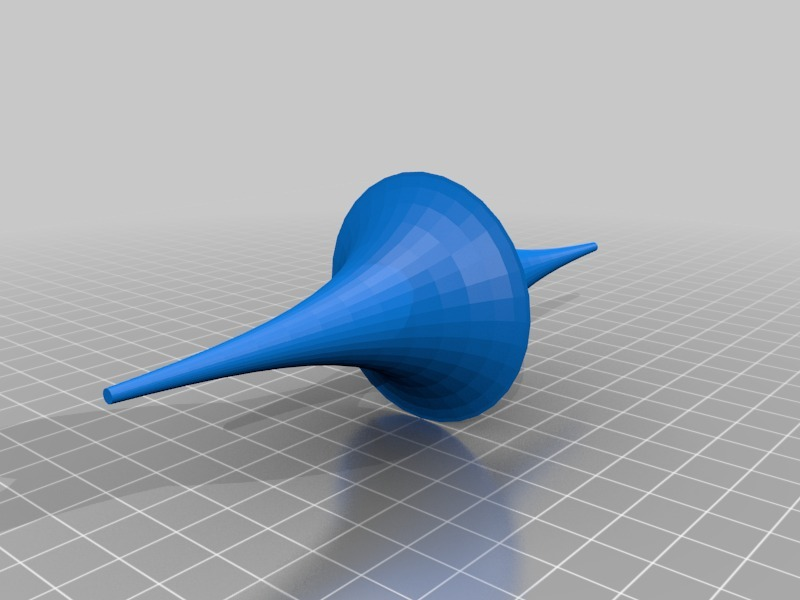
\includegraphics[width= 1\linewidth]{Pseudosphere.jpg}
		\caption{\small\textit{\color{lichsutoanhoc}Mặt giả cầu (pseudosphere).}}
		\vspace*{-10pt}
	\end{figure}
	Lúc này ta càng phải trân trọng sự thiên tài của Euclid. Ông không những xếp đây là tiên đề sau cùng, mà còn hoãn việc dùng đến nó trong tận $29$ kết quả đầu tiên trong ``Elements". Những gì mà tận hai thiên niên kỷ sau mới phát hiện là bảo chứng cho tính độc lập của tiên đề thứ $5$: nó không thể là một định lý rút ra từ chỉ $4$ tiên đề đầu tiên. Tiên đề thứ $5$ thật sự là một tiên đề độc lập.
	\vskip 0.1cm
	Lộn lại vấn đề về gốc rễ, xét mệnh đề phủ định của Tiên đề $5$ theo phát biểu của Playfair:
	\vskip 0.1cm
	Tiên đề $5$: Cho trước $1$ điểm $M$ không nằm trên $d$, có đúng một đường thẳng $d'$ đi qua $M$ và song song với $d$
	\vskip 0.1cm
	sẽ có phủ định là: 
	\vskip 0.1cm
	Tồn tại một điểm $M$ và đường thẳng $d$ không đi qua nó, sao cho số đường thẳng đi qua $M$ và song song với $d$ là khác $1$. Con số này có thể là $0$ hoặc ít nhất $2$. 
	\vskip 0.1cm
	Hóa ra, trường hợp thứ hai tương đương với giả thuyết góc nhọn vững chãi mà Saccheri đã không loại được. Còn trường hợp con số ấy là $0$, nói cách khác là mọi đường thẳng đều giao nhau, thì vị tu sĩ của chúng ta đã loại ngon ơ rồi mà. Đồng thời, Định lý $16$ (định lý góc ngoài) và  Định lý $27$ (định lý góc so le trong) trong \textit{Cơ sở} của Euclid đã chỉ ra sự tồn tại của đường song song kia mà.
	\vskip 0.1cm
	Thực ra, cánh cửa mà ta tưởng như Saccheri đã khóa kín cũng ẩn chứa trong nó một thế giới phong phú khác, gọi là hình học elliptic. Sau này, Riemann và những đóng góp của ông đã thống nhất và đào sâu hơn vào cả hình học elliptic và hình học hyperbolic, nội dung những đóng góp này xin hẹn độc giả ngày nào đó không xa. Còn điều vô lý ta vừa chỉ ra thực chất có thể truy ngược về một trong các giả định được ngầm thừa nhận.
	\vskip 0.1cm
	\textbf{Tài liệu tham khảo}
	\vskip 0.1cm
	[$1$] E.T.  Bell, \textit{Men of Mathematics The Lives and Achievements of the Great Mathematicians from Zeno to Poincaré}.   
	\vskip 0.1cm
	[$2$] David M. Burton. \textit{The History of Mathematics An Introduction}. 
	\vskip 0.1cm
	[$3$] M. J. Greenberg, \textit{Euclidean and Non--Euclidean Geometries -- Development and History}. 
	\vskip 0.1cm
	[$4$] Wikipedia tiếng Anh.
	\vskip 0.1cm
	[$5$] \url{https://www.youtube.com/playlist?list} \url{=PLjLK2cYtt-VBSBtvfhxx-DW3Zw3nOQ}\\
	\url{HVZ}  
	\vskip 0.1cm
	[$6$] \url{https://rosetta.vn/lequanganh/wp-cont}\\
	\url{ent/uploads/sites/7/2018/07/Riemann.pdf} 
	\vskip 0.1cm
	[$7$] \url{https://www.cut-the-knot.org/triangle/pythpar/Drama.shtml}
	\end{multicols}